\documentclass[tikz,border=3mm]{standalone}
\usepackage{amsmath}
\usetikzlibrary{arrows.meta,positioning,shapes.geometric,fit,backgrounds}
\begin{document}
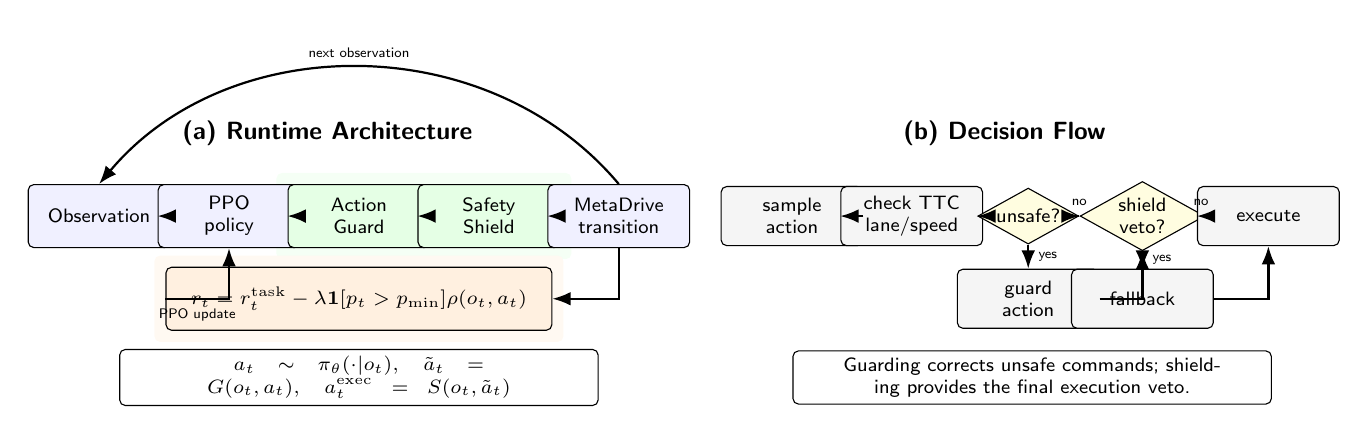
\begin{tikzpicture}[font=\sffamily, >=Latex,
box/.style={draw, rounded corners=2pt, fill=blue!6, minimum width=18mm, minimum height=8mm, align=center, font=\sffamily\scriptsize},
safe/.style={draw, rounded corners=2pt, fill=green!10, minimum width=18mm, minimum height=8mm, align=center, font=\sffamily\scriptsize},
risk/.style={draw, rounded corners=2pt, fill=orange!12, minimum width=49mm, minimum height=8mm, align=center, font=\sffamily\scriptsize},
flow/.style={draw, rounded corners=2pt, fill=gray!8, minimum width=18mm, minimum height=7.5mm, align=center, font=\sffamily\scriptsize},
decide/.style={draw, diamond, aspect=1.8, fill=yellow!12, inner sep=0.8pt, align=center, font=\sffamily\scriptsize},
formula/.style={draw, rounded corners=2pt, fill=white, inner sep=2.5pt, align=center, font=\sffamily\scriptsize}]

\node[font=\sffamily\bfseries\small] at (-3.45,1.05) {(a) Runtime Architecture};
\node[box] (obs) at (-6.35,0) {Observation};
\node[box] (ppo) at (-4.70,0) {PPO\\policy};
\node[safe] (guard) at (-3.05,0) {Action\\Guard};
\node[safe] (shield) at (-1.40,0) {Safety\\Shield};
\node[box] (env) at (0.25,0) {MetaDrive\\transition};
\node[risk] (risk) at (-3.05,-1.05) {$r_t=r_t^{\rm task}-\lambda\mathbf{1}[p_t>p_{\min}]\rho(o_t,a_t)$};
\node[formula, text width=59mm] (eq) at (-3.05,-2.05) {$a_t\sim\pi_\theta(\cdot|o_t),\quad \tilde a_t=G(o_t,a_t),\quad a_t^{\rm exec}=S(o_t,\tilde a_t)$};
\draw[->, thick] (obs) -- (ppo);
\draw[->, thick] (ppo) -- (guard);
\draw[->, thick] (guard) -- (shield);
\draw[->, thick] (shield) -- (env);
\draw[->, thick, rounded corners=8pt] (env.north) to[out=130,in=50] node[above,font=\sffamily\tiny] {next observation} (obs.north);
\draw[->, thick] (env.south) |- (risk.east);
\draw[->, thick] (risk.west) -| node[pos=0.25,below,font=\sffamily\tiny] {PPO update} (ppo.south);
\begin{scope}[on background layer]
\node[fill=green!4, rounded corners=2pt, fit=(guard)(shield), inner sep=4pt] {};
\node[fill=orange!5, rounded corners=2pt, fit=(risk), inner sep=4pt] {};
\end{scope}

\node[font=\sffamily\bfseries\small] at (5.15,1.05) {(b) Decision Flow};
\node[flow] (sample) at (2.45,0) {sample\\action};
\node[flow] (check) at (3.97,0) {check TTC\\lane/speed};
\node[decide] (unsafe) at (5.45,0) {unsafe?};
\node[flow] (gact) at (5.45,-1.05) {guard\\action};
\node[decide] (veto) at (6.90,0) {shield\\veto?};
\node[flow] (exec) at (8.50,0) {execute};
\node[flow] (fallback) at (6.90,-1.05) {fallback};
\node[formula, text width=59mm] at (5.50,-2.05) {Guarding corrects unsafe commands; shielding provides the final execution veto.};
\draw[->, thick] (sample) -- (check);
\draw[->, thick] (check) -- (unsafe);
\draw[->, thick] (unsafe) -- node[above,font=\sffamily\tiny] {no} (veto);
\draw[->, thick] (unsafe) -- node[right,font=\sffamily\tiny] {yes} (gact);
\draw[->, thick] (gact.east) -| (veto.south);
\draw[->, thick] (veto) -- node[above,font=\sffamily\tiny] {no} (exec);
\draw[->, thick] (veto) -- node[right,font=\sffamily\tiny] {yes} (fallback);
\draw[->, thick] (fallback.east) -| (exec.south);
\end{tikzpicture}
\end{document}
